\section{Results}
This project was mostly exploratory; we envision a previously unaddressed type of intermittent bug that can theoretically exist, develop a static analysis tool to detect the relevant code pattern, and then see if compelling examples actually exist in the wild. They do, particularly in sensor drivers and low-level client applications. For our results, we present three case studies: one taken from the TI-RTOS magnetometer driver, and two taken from example software applications bundled with TI-RTOS. For each case, we give the simplified source code, annotated with a restart and power failure point that triggers the bug, the program execution trace, and a discussion of the possible consequences of each bug.

\subsection{The Magnetometer Driver}

Figure \ref{fig:mag} shows the initialization function of the magnetometer driver, with the simplfied source code on the right and the buggy execution trace on the left. The function checks that the sensor is powered on and conditionally reads from the I2C bus. If the read was successful, the raw data from the bus read is stored into the X, Y, Z fields of the calibration structure, and if the read was not successful the function simply returns. 
\begin{figure}[h]
\centering
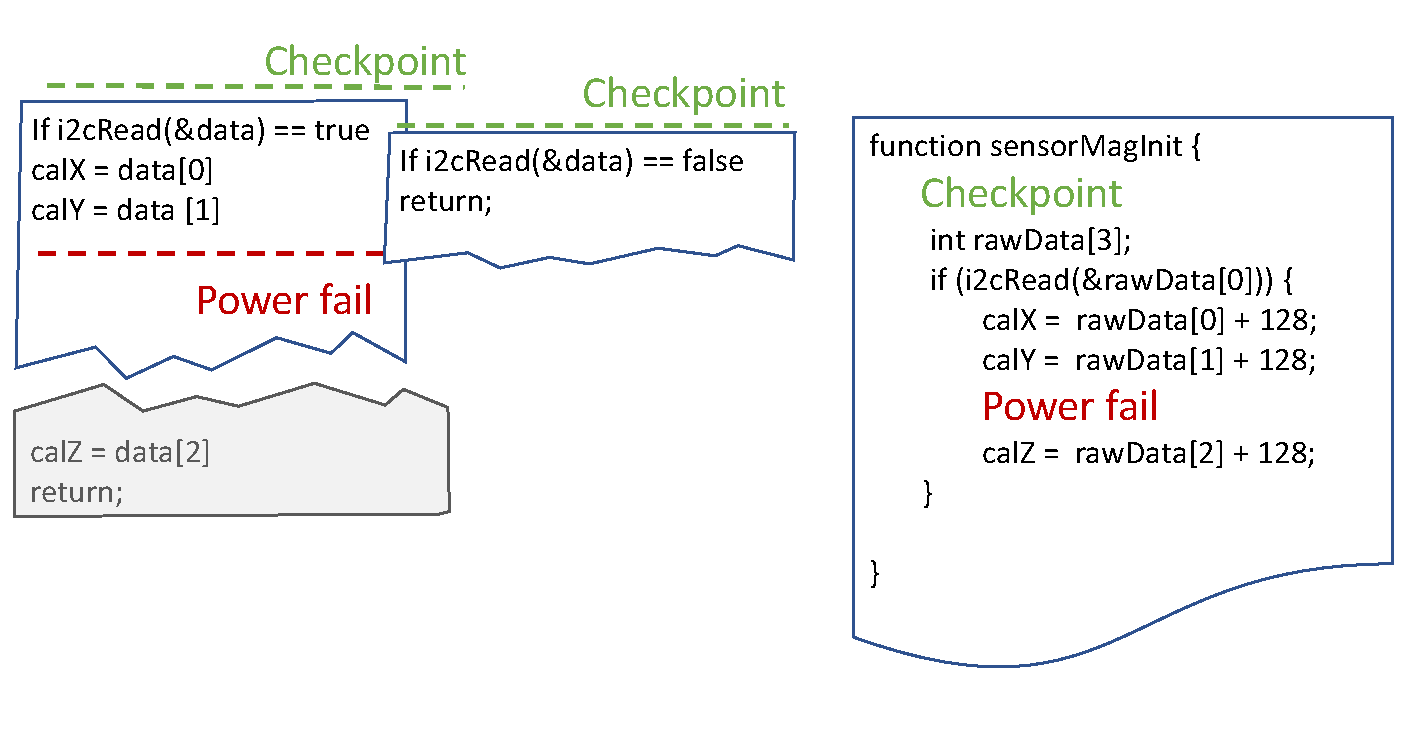
\includegraphics[width=1\columnwidth]{maginit_bug.pdf}
\caption{Bug in magnetometer initialization. Power failing while updating the calibration fields can cause the calibration data to become inconsistent, corrupting any future magnetometer reads that use the calibration.}
\label{fig:mag}
\end{figure}

Non-idempotent I/O enters the program at the I2C read, from both the return value and the actual raw data, and in this case the program branches on the return value. A buggy execution is possible if we latch execution state at the beginning of the function and read successfully from the bus. Since the read returned true, we take the branch, and begin storing the raw data into the calibration fields. In this particular execution, the device runs out of power and fails after writing to calY. The write to calZ, in the greyed-out portion of the trace, is not reached. On reboot, execution resumes from the top of the function, but on this execution the read from the bus fails, introducing the I/O non-idempotency into the program. The branch is not taken, and the function returns, leaving the calibration data in a state unreachable on continuous execution - two fields are set with the correct data, but the third has some unknown default value. 
Since this is a device driver, any higher level applications that read data from the magnetometer will filter it through these corrupted, inconsistent calibration fields, possibly leading to wildly incorrect application behavior or crashes.  

\subsection{Wireless Sensor Node Concentrator}

Figure \ref{fig:wsn} shows the main task loop of an aggregator node and the called updateNode function, with the simplfied source code on the right and the buggy execution trace on the left. This code is part of a larger application that receives RF packets from sensor nodes and stores the node adc, rssi, and data into a list, adding the node if it wasn't already in the list. 

\begin{figure}[h]
\centering
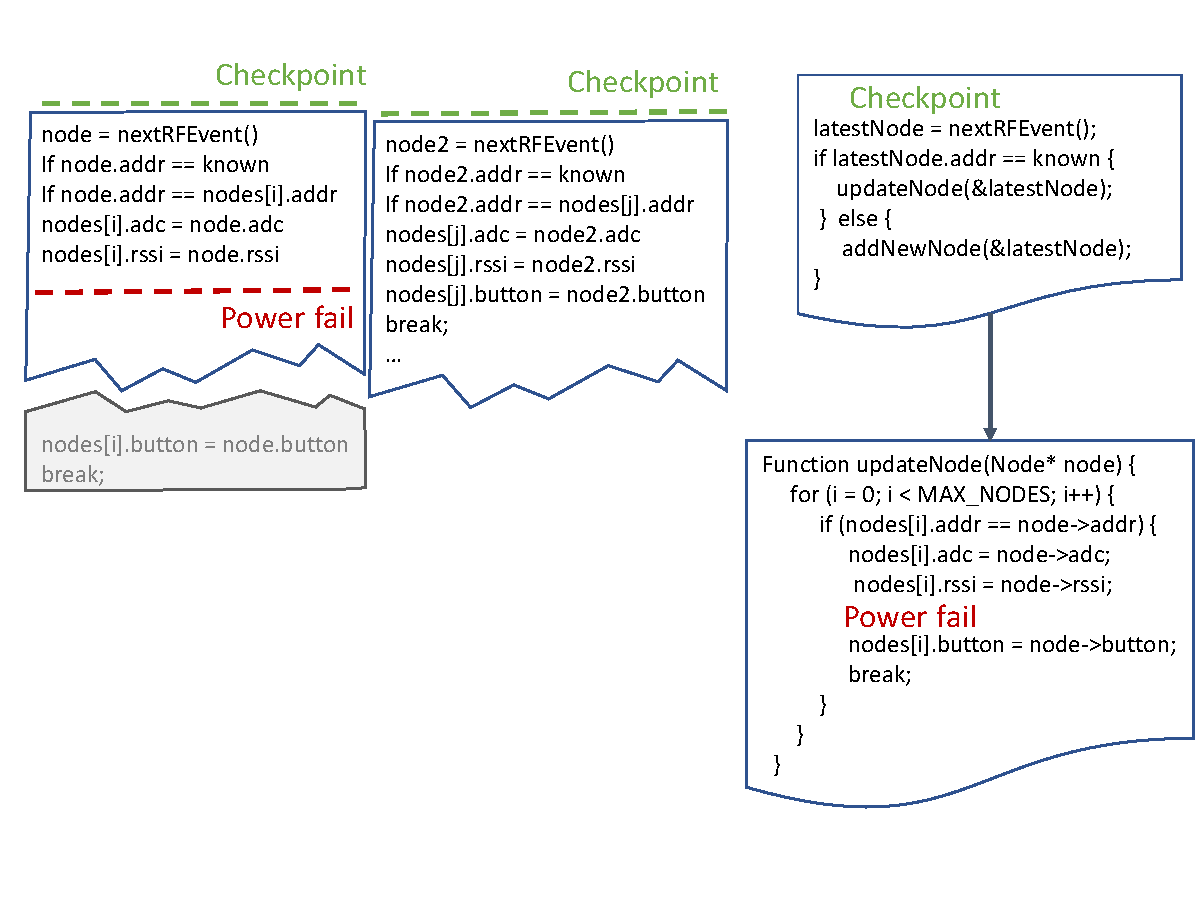
\includegraphics[width=1\columnwidth]{wsn_concentrator_bug.pdf}
\caption{Bug in WSN concentrator. Power failing while updating the node structure can cause the node list to become inconsistent, corrupt the payload ("button" field) or use out-of-date timing information, possibly messing up system protocols}
\label{fig:wsn}
\end{figure}

Non-idempotent I/O enters the program through the received packet, which could come from a different node each time. In the buggy execution trace displayed, the program latches execution at the top of the task loop, before receiving a packet. Upon receiving the packet, it checks that this is a node that has been seen before and calls the updateNode function. UpdateNode determines the identity of the node (in this case the node at nodes[i]) and starts updating the node fields. This branch within updateNode is the I/O tainted branch. As in the last example, power fails before it finishes updating all the fields, leaving the payload (which button was pushed) update unexecuted. On reboot, the next packet has come from a different node - the node at nodes[j] - whose fields get all updated, and the program continues with its task loop, dropping the first node's data. Losing data is perhaps not a catastrophic consequence, but it does leave the node state inconsistent and can lead to incorrect program behavior. Additionally, the state between the sending sensor node and this receiver is corrupted, since the sending node will see that the receiver correctly received the packet, but the receiver nodes internal structures did not fully update with the new information.

\subsection{RF EasyLink Receiver}
Figure \ref{fig:rf} shows the EasyLink receive function, with the simplfied source code on the right and the buggy execution trace on the left. EasyLink is a simpler API sitting on top of the base RF driver. In this function, there is a status variable, initialized to Error at the beginning of the program, that tracks whether or not packets conform to the EasyLink protocol, and there is result variable that checks whether or not the packet was received correctly. If the packet is received correctly, the function checks if the data was completed, setting status to error if not. If the packet status is ok, the function further checks that the statistics received from the event queue are correct, and then finally begins updating the local packet structure with the received data, setting the status variable to success.
\begin{figure}[h]
\centering
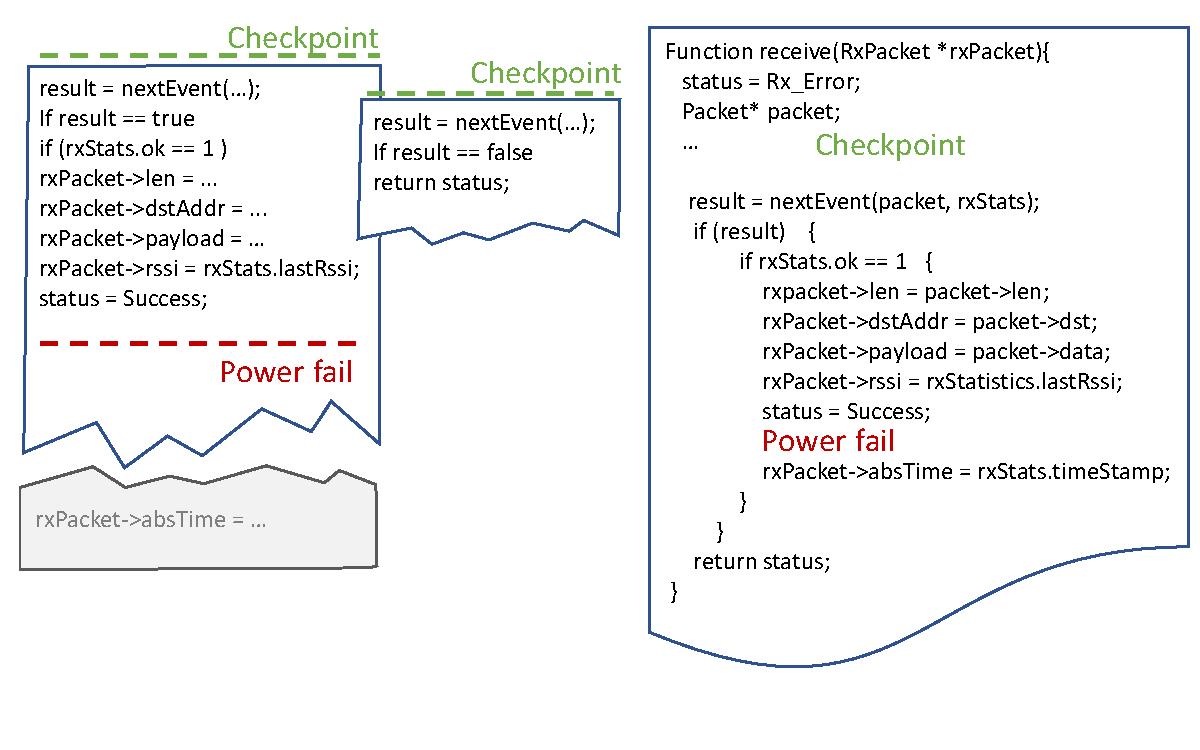
\includegraphics[width=1\columnwidth]{easylinkrx_bug.pdf}
\caption{Bug in RF EasyLink Receiver. Power failing before returning a correctly read packet can cause the status field to be set to success, even if the next event fails. The function will return an incorrect status value, potentially crashing the larger application.}
\label{fig:rf}
\end{figure}

Non-idempotent I/O again enters the program both through the received packet and the return value of the receivePacket call, and so the branch on result is also non-idempotent. In the buggy trace, execution is latched right before receiving the packet. On the first execution, the packet is good; it passes all the checks and updated the local packet variable, setting the status to success. Power then fails. On reboot and re-execution, the next packet is not received correctly, causing the branch on result to not be taken. The function, however, just returns the status variable, which is still set to success, as on continuous execution there is no path where success can be true and result can be false. Thus, even though the most recent packet event failed, the receive function still returns success. Additionally, not all the fields of the original, good packet are updated.
The bug from this program is highly dependent on where the programmer puts the checkpoints - putting it right before the I/O call is reasonable, particularly if receiving and processing the I/O is expensive, and the programmer wants a fully energy buffer on reboot. On the other hand, if the programmer uses a task-based latching model, such as Alpaca \cite{alpaca}, and this entire function becomes one task, the bug disappears, since status will always be reinitialized to error. 
 
